\chapter{通信网结构}
\section{图论基础}
\subsection{一笔画问题}
\textbf{奇点:}与该条边连接的个数有奇数个\\
\textbf{偶点:}与该条边连接的个数有偶数个\\
一笔画定理:
\begin{itemize}
	\item 中间点一定是偶数点
	\item 最多有两个奇点
	\item 若由偶点组成的连通图,一定可以一笔画,以任意点为起点一以这个点为终点
	\item 只有两个奇点的连通图,一定可以一笔画完;画时以一个奇点为起点,另一个奇点为终点。
\end{itemize}
\subsection{图的基础知识}
\subsubsubsection{基础概念}
\begin{itemize}
	\item 相邻点: vi与vj 互为相邻点( vi 和vj 是一条边的两个端点)
	\item 相邻边:两条边与同一端点相关联,则这两条边为相邻边
	\item 度数(或次数):与同一端点相关联的边的个数
	\item 两个端点重合为一点的边成为自环。
	\item 并行边,与同一队端点关联的两条边或两条以上的边
	\item 简单图与复杂图,没有自环和并行边的图称为简单图,否则称为复杂图
	\item 空图:没有点
	\item 孤立点:有点但无边
	\item 平面图和非平面图:非平面图画在平面上时,至少有两条边要相交。平面图则不想交	
\end{itemize}
\subsubsubsection{图的运算}
\begin{itemize}
	\item 并图
	\begin{figure}[H]
		\centering
		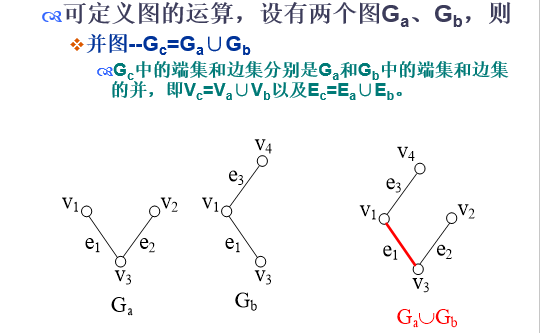
\includegraphics[width=0.5\linewidth]{figures/screenshot039}
		\caption{}
		\label{fig:screenshot039}
	\end{figure}
	\item 交图 
	\begin{figure}[H]
		\centering
		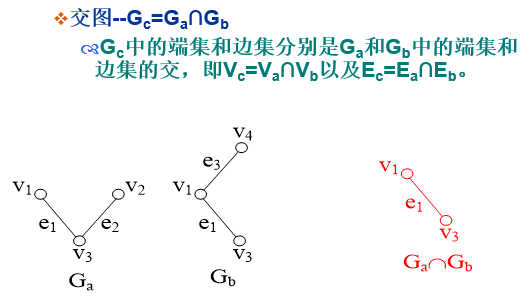
\includegraphics[width=0.5\linewidth]{figures/screenshot040}
		\caption{}
		\label{fig:screenshot040}
	\end{figure}
	\item 差图
	 \begin{figure}[H]
		\centering
		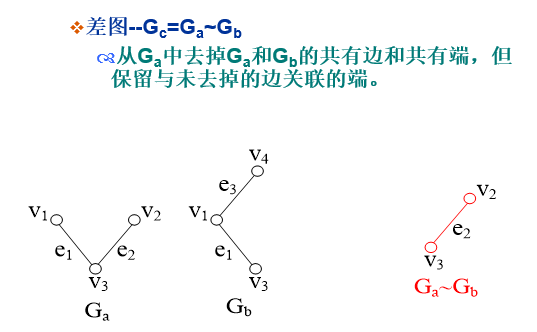
\includegraphics[width=0.7\linewidth]{figures/screenshot041}
		\caption{}
		\label{fig:screenshot041}
	\end{figure}
	一般来说:$ G_a ~ G_b = G_a - G_a\cap G_b $ ,所以该运算要分方向
	\item 环合图
	\begin{figure}[H]
		\centering
		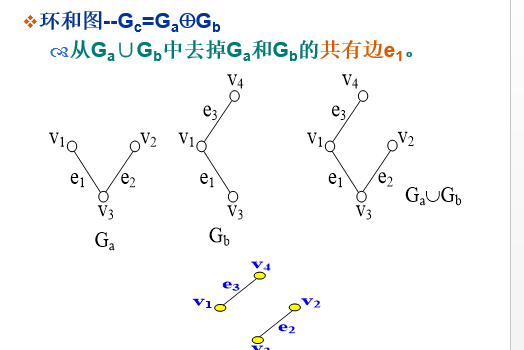
\includegraphics[width=0.7\linewidth]{figures/screenshot042}
		\caption{}
		\label{fig:screenshot042}
	\end{figure}
\end{itemize}
\subsubsection{图的联结性}
\begin{description}
	\item[1.端的度数] 与端相关的变数为该端的度数,自环度数+2.在有向图中\textbf{$ d^+(v_i) $表示离开}$ v_i $的边数,\textbf{$ d^-(v_i) $表示进入},$ v_i $的度数。
\end{description}
\textbf{图的度数性质:}
对于有n个端,m条边的无向图
\begin{equation}\label{key}
\sum_{i=1}^{n}d(v_i) = 2m
\end{equation}
若G为有向图
\begin{equation}\label{key}
\sum_{i=1}^{n}d^+(v_i) = \sum_{i=1}^{n}d^-(v_i) = m
\end{equation}
任意图中,\textbf{度为奇数数的端的数目必为偶数}。
\subsubsection{链、径和还}
\begin{description}
	\item[边序列] 有限条边的一种串序排列称为边序列,要求相邻两边有公共端。(边可重复)
	\item [链] 没有重复边的链
	\item [环] 起点和终点为同一端的链
	\item[径] 无重复边、无重复端的边序列
\end{description}
\subsubsection{连接图}
\textbf{联结图的一般定义}:图内任何2个端之间至少有一条径,这图就称为联结图(或称连通图)。否则就是非联结图(或非连通图)\\
非连接图总可以分为几个部分,所谓部分是指原图的一个子图,该子图\textbf{是一个最大连接图}
\begin{figure}[H]
	\centering
	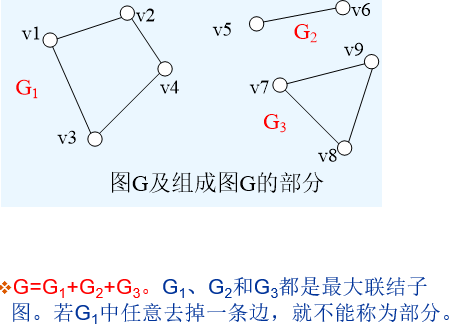
\includegraphics[width=0.7\linewidth]{screenshot003}
	\caption{}
	\label{fig:screenshot003}
\end{figure}
\subsubsection{几种特殊的连接图}
\begin{enumerate}
	\item \textbf{全连接图}:任意两端都有边的无向图成为全连接图各端的度数均为d(vi)=n-1,。其边m和端n的关系
	\begin{figure}[H]
		\centering
		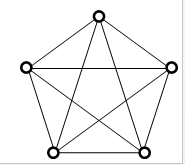
\includegraphics[width=0.3\linewidth]{figures/screenshot046}
		\caption{}
		\label{fig:screenshot046}
	\end{figure}
	
	\begin{equation}\label{key}
	m = C_n^2 = \frac{n(n-1)}{2}
	\end{equation}
	\item \textbf{两部图}:端点集合可分为2个部分,所有边的2个邻端分别在这2个集合中。特别,\textbf{完全两部图}Km,n的端点集合有2个部分,分别有m和n个端点;从2个端集合中各任取一个端,它们之间都有一条边,共有mn条边。
	\begin{figure}[H]
		\centering
		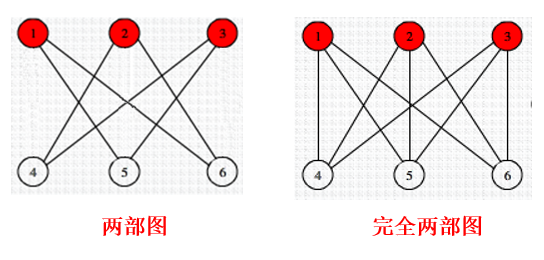
\includegraphics[width=0.7\linewidth]{figures/screenshot047}
		\caption{}
		\label{fig:screenshot047}
	\end{figure}
	
	\item 正则图:所有段的度数都相等.正则图的联结性最均匀;无重边和自环的全联结图是正则图。
	\begin{figure}[H]
		\centering
		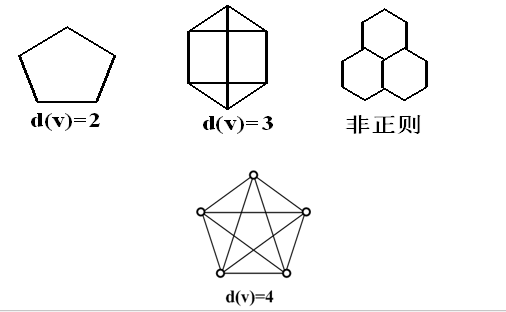
\includegraphics[width=0.7\linewidth]{figures/screenshot048}
		\caption{}
		\label{fig:screenshot048}
	\end{figure}
	
	\item 欧拉图:端度数均为偶数(不一定为连接图)。\\
连接欧拉图<=>存在一个含全边的环	
\begin{figure}[H]
	\centering
	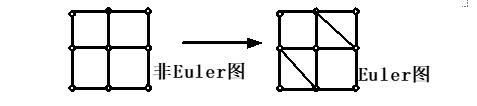
\includegraphics[width=0.7\linewidth]{figures/screenshot049}
	\caption{}
	\label{fig:screenshot049}
\end{figure}
	\begin{figure}[H]
		\centering
		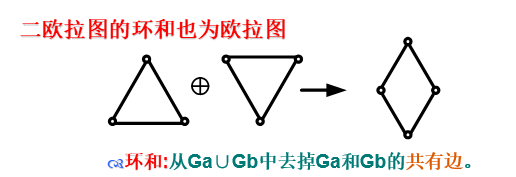
\includegraphics[width=0.7\linewidth]{figures/screenshot050}
		\caption{}
		\label{fig:screenshot050}
	\end{figure}
	
	\item M图:如果图中只有2个度数为奇数的端,则此图称为M图。\\
	M图可以是联结图,也可以是非联结图,但此时各部分除一个是M图外,其他都是欧拉图。
	\begin{figure}[H]
		\centering
		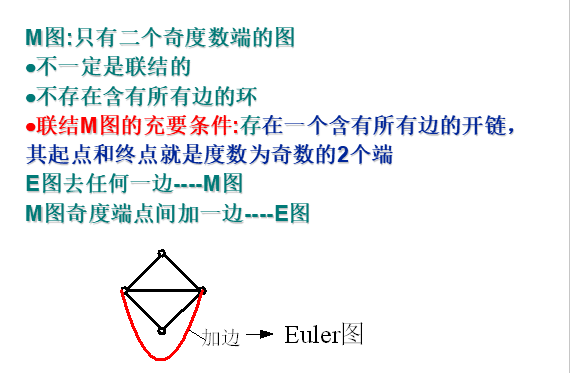
\includegraphics[width=0.7\linewidth]{figures/screenshot051}
		\caption{}
		\label{fig:screenshot051}
	\end{figure}
	
	\item 汉密尔顿(Hamilton)图:当图中至少存在一个含有所有端的环,这个图称为汉密尔顿图(也称哈密顿图),上述的环称为汉密尔顿环。
	\begin{figure}[H]
		\centering
		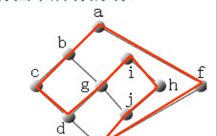
\includegraphics[width=0.7\linewidth]{figures/screenshot052}
		\caption{}
		\label{fig:screenshot052}
	\end{figure}
	
\end{enumerate}

\section{树}
定义:任何二端间有径且只有一条径的图
\subsection{基本性质}
\begin{enumerate}
	\item 树是无环的连接图
	\item 树是最小连通图。去掉任意一边就变成非连接图
	\item 若树有m条边及n个端,则有\textbf{m=n-1}
	\item 除单点树外,树\textbf{至少有2个端的度数为1}
\end{enumerate}
\subsection{树的一些概念}
\begin{figure}[H]
	\centering
	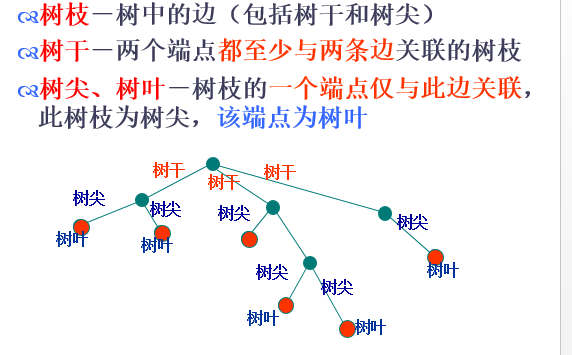
\includegraphics[width=0.7\linewidth]{figures/screenshot053}
	\caption{}
	\label{fig:screenshot053}
\end{figure}

\subsection{主树}
生成树:包含所有端点,\textbf{一定为连通图},可能不止一个
\subsection{树枝与连枝}
对于图的某一棵主树而言,主树上的边称为树枝,非树枝的边称为连枝。
主树就是树枝集;
连枝的边集称为连枝集或称为树补。
\subsection{图G的阶及其空度
}
\subsubsection{阶}
联结图G的主树T的树枝数称为图G的阶。
若图G有n个端,则它的阶$ \rho $为
$ \rho $(G)=$ \rho$=| T|=mT=n-1
\subsubsection{空度}
联结图G的连枝集的连枝数称为图G的空度,记为$ \mu $。
当G有m条边时,有\textbf{$  \mu(G)=|G-T|=m-n+ $1} 且 $ \rho+\mu=m $
\begin{itemize}
	\item $ \mu $越大,连枝数越多,图G的联结性越好。
	\item $ \mu = 0 $表示最低联结性,即G是最小连接图。
\end{itemize}
\subsubsection{主林与林补}
对一个非联结图G,它可分成k个部分,也就是k个最大联结图。每个部分至少有一棵主树。这可找到k棵主树,所形成的集称为主林。余下的边所形成的集称为林补。
此时,G的阶可定义为主林的边数,G的空度为林补的边数。
\begin{equation}\label{key}
\rho(G)=(n1-1)+(n2-1)+….+(nk-1)=n-k 
\end{equation}
\begin{equation}\label{key}
\mu(G)=m-n+k \\
\end{equation}

\section{割和环}
\subsection{割}
割是指图的某些子集,\textbf{去掉这些子集就使图的部分数增}加。若图是联结的,去掉这种子集就成为非联结图。\\
根据这种子集的元素不同,可分为割端集和割边集。
\subsubsection{割端与割端集}
\subsubsubsection{割端}
\textbf{割端:}令v是G的一个端,在去掉v和与之关联的边后,若使G的部分数增加,则称v是G的割端。
\subsubsubsection{割端集}
\textbf{割端集}:去掉几个端后,部分数增加,则这些端的集称为割端集。\\
\textbf{最小割端集中的端数},称为图的联结度,表示要破坏图的联结性的难度;联结度愈大,联结性愈不易被破坏。
\subsubsection{割边集和割集}
\textbf{割边集}:令S是联结图G的边子集,如果在G中去掉S能使G成为非联结图,则称S是G的割边集\\
\textbf{割集,最小割边集}:\textbf{若S的任何真子集都不是割边集},称S是割集。
实际上\textbf{,割集是最小割边集}。\\
\textbf{最小割集的边数称为图的结合度,表示图的联结程度。}
\begin{figure}[H]
	\centering
	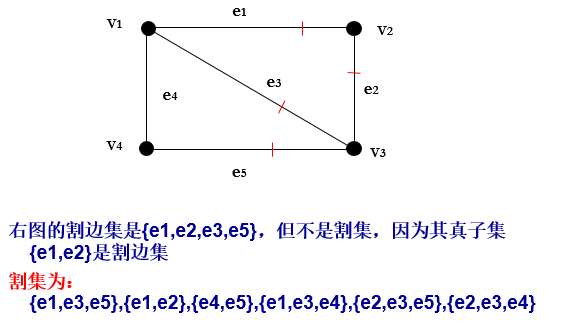
\includegraphics[width=0.7\linewidth]{figures/screenshot054}
	\caption{}
	\label{fig:screenshot054}
\end{figure}

\subsection{联结度、结合度、连通度}
\begin{itemize}
	\item 联结度:最小割端集的端数称为图的联结度。
	\item 结合度:最小割集的边数称为图的结合度。
	\item 连通度:联结度和结合度统称为连通度。
\end{itemize}
\textbf{联结度是点连通度;
结合度是边连通度}
对于通信网来说,连通度越高,可靠性越好
\subsection{基本割集}
设T是联结图G的一棵主树,取一条树枝与\textbf{某些连枝}一定能构成一个割集,这种割集称为基本割集。\\
\textbf{基本割集只含一条树枝}\\
若G有n个端,则主树有n-1条树枝,所以有$ n-1 $个基本割集\\
基本割集有$ n-1 $,由基本割集及其\textbf{环和}共形成$ 2^(n-1)-1 $(二项式求和),然后排除重复的地方。                                \begin{figure}[H]
	\centering
	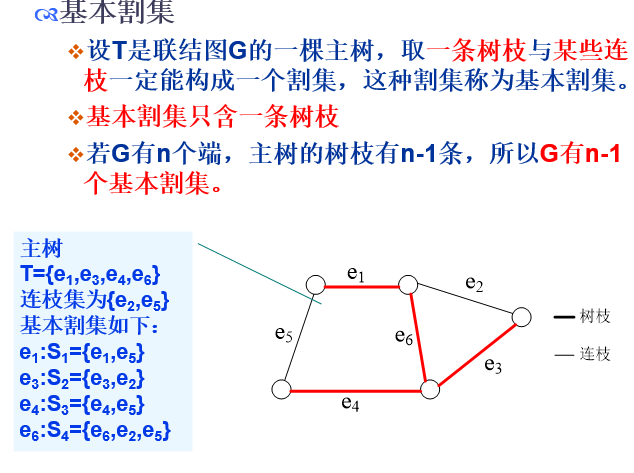
\includegraphics[width=0.7\linewidth]{figures/screenshot045}
	
	\caption{}
	\label{fig:screenshot045}
\end{figure}
\begin{figure}[H]
	\centering
	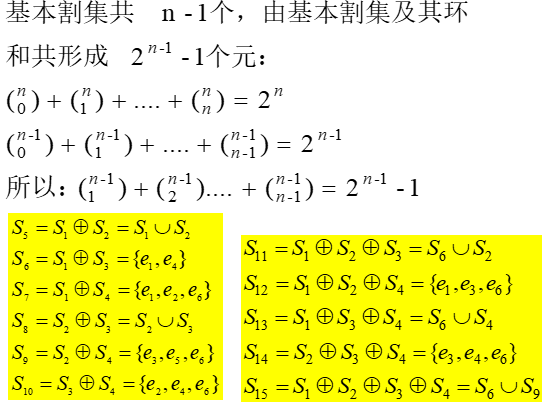
\includegraphics[width=0.7\linewidth]{figures/screenshot056}
	\caption{}
	\label{fig:screenshot056}
\end{figure}
\begin{enumerate}
	\item $ C_4^1 $
		\item $ C_4^2 $
			\item $ C_4^3 $
				\item $ C_4^4 $
\end{enumerate}
\textbf{再去掉所有基本割集的并或者重复的。}
 \subsection{基本环和所有环的方法}                              
取一条连枝可与某些树枝构成\textbf{闭径或环}。这种仅包含有一条连枝的环称为联结图的\textbf{基本环}。显然,基本环的数目等于连枝数\textbf{m-n+1}。
基本环的环和可组成$ 2^{m-n+1}-1 $个元,每个元或为环,或为环的并。
\begin{figure}[H]
	\centering
	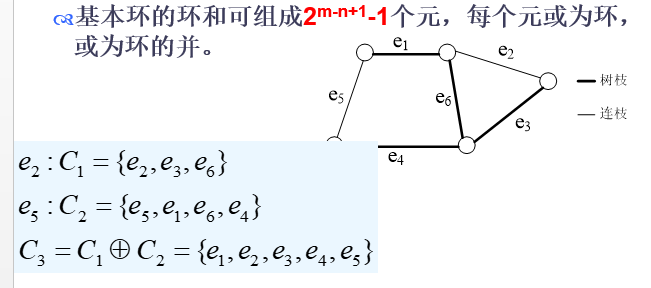
\includegraphics[width=0.7\linewidth]{figures/screenshot044}
	\caption{}
	\label{fig:screenshot044}
\end{figure}

\section{平面性和对偶性}
平面图,任意两条边无交点(除端点)。
\subsection{平面型}
\begin{itemize}
	\item 设一个联结的平面图有m条边,n个端,把平面分成S个区域(包括开区域),它们之间有$ S=m-n+2 $。
	\item 对于无重边、无自环的联结图,具有平面性的必要条件是$ m\le 3n-6 $(即平面图必定有$ m\le 3n-6 $ ,但$ m\le 3n-6 $ 不一定是平面图)。
\end{itemize}
\subsection{对偶性}
设有两个边集E相同的图G1和G2,若G2中每个无重复端的环(闭径)都对应G1中的一个割集,反之亦然,则G1和G2互为对偶图或具有对偶性。
\begin{itemize}
	\item \textbf{平面图的对偶图总是存在的,而非平面图是没有对偶图的}。
	\item 倘若一个图G的对偶图就是自己,则称G为自对偶图。
	
\end{itemize}
\begin{figure}[H]
	\centering
	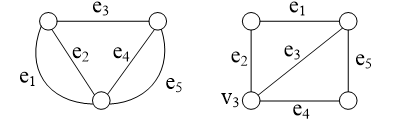
\includegraphics[width=0.7\linewidth]{figures/screenshot057}
	\caption{}
	\label{fig:screenshot057}
\end{figure}
\begin{figure}[H]
	\centering
	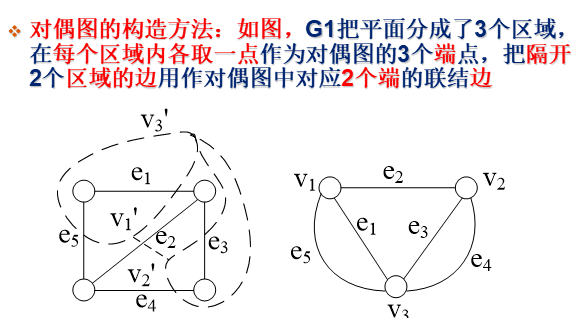
\includegraphics[width=0.7\linewidth]{figures/screenshot058}
	\caption{}
	\label{fig:screenshot058}
\end{figure}
\section{图阵}
\subsection{关联阵}
\subsubsection{全关联阵}
\begin{figure}[H]
	\centering
	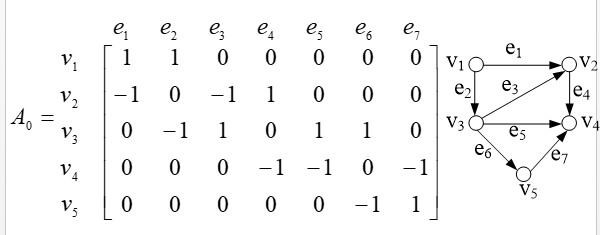
\includegraphics[width=0.7\linewidth]{figures/screenshot060}
	\caption{}
	\label{fig:screenshot060}
\end{figure}
\begin{figure}[H]
	\centering
	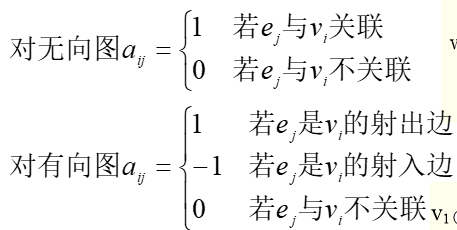
\includegraphics[width=0.7\linewidth]{figures/screenshot061}
	\caption{}
	\label{fig:screenshot061}
\end{figure}
\begin{itemize}
	\item 每行中非零元素的个数等于该端的度数
	\item 每一列元素之和为对无向图为2,对有向图为0
\end{itemize}
\subsubsection{关联阵}
\textbf{去掉全关联阵中的任一行即得关联阵}
\begin{itemize}
	\item 联结图的关联矩阵中,必存在至少一个(n-1) ×(n-1)的方阵是非奇异的,这个方阵所对应的边集就是一棵主树。
	\item 若关联矩阵中有一个(n-1) ×(n-1)的方阵是奇异的,即它的行列式值为零,则这方阵所对应的边集中必存在环。
	\item 当关联矩阵的阶小于n-1时,它所对应的图必为非联结图,因为没有(n-1) ×(n-1)的方阵是非奇异的,也就是不存在主树。
\end{itemize}
\textbf{联结图主树数目S与全关联阵的关系
}\begin{equation}\label{key}
S = |AA^T|
\end{equation}
\begin{figure}[H]
	\centering
	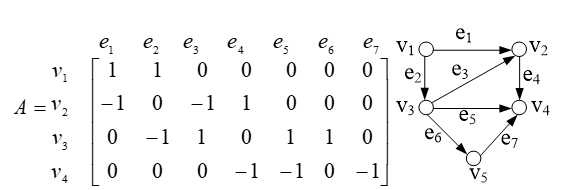
\includegraphics[width=0.7\linewidth]{figures/screenshot062}
	\caption{}
	\label{fig:screenshot062}
\end{figure}
\begin{itemize}
	\item AAT(无重复边)对角线上的元是端的度数(A0中没有删的行所对应的端),其他元非-1即零(若两个端之间没有边,为零,有边为-1)。
	\item 对于无向图,可以在图上任意加箭头,得相应的有向图,这样就可以求得无向图的主树数目.
\end{itemize}
\subsection{割阵}
\begin{figure}[H]
	\centering
	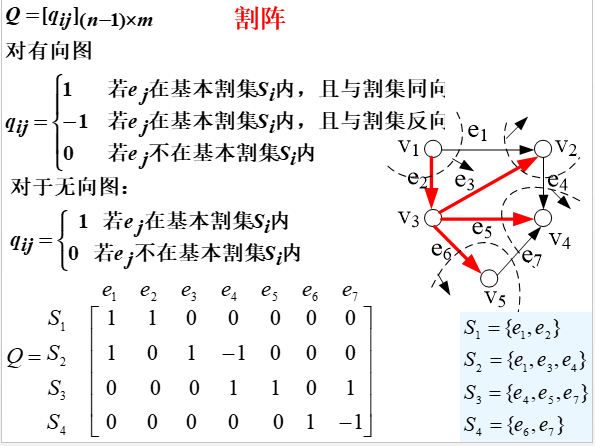
\includegraphics[width=0.7\linewidth]{figures/screenshot064}
	\caption{}
	\label{fig:screenshot064}
\end{figure}
S1,S2,S3,S4为基本割集。\textbf{正负1看树枝所指端,如果边枝和树枝指向相同则为正,反之为负}
\begin{figure}[H]
	\centering
	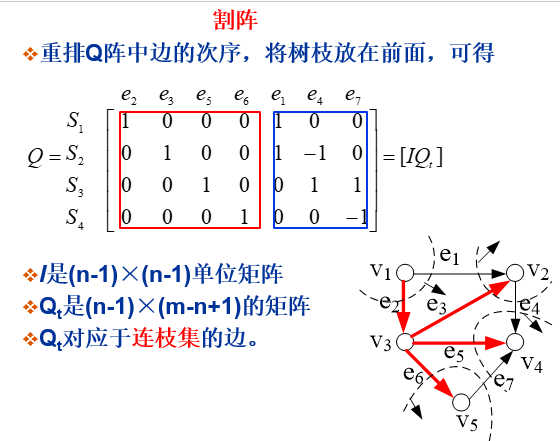
\includegraphics[width=0.7\linewidth]{figures/screenshot065}
	\caption{}
	\label{fig:screenshot065}
\end{figure}
\begin{figure}[H]
	\centering
	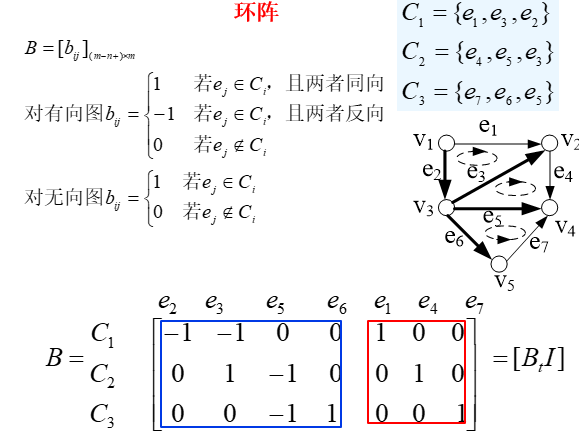
\includegraphics[width=0.7\linewidth]{figures/screenshot066}
	\caption{}
	\label{fig:screenshot066}
\end{figure}
\textbf{联结图的环阵B和割阵Q以下关系,若边的次序是一样的: $ BQ^T $=0
}
\subsection{邻接阵}
\begin{figure}[H]
	\centering
	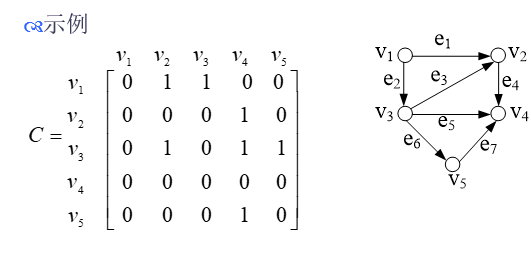
\includegraphics[width=0.7\linewidth]{figures/screenshot067}
	\caption{}
	\label{fig:screenshot067}
\end{figure}
\section{最短径问题}
\subsection{最短主树}
\subsubsection{无限制条件}
\subsubsubsection{P算法
}
\begin{figure}[H]
	\centering
	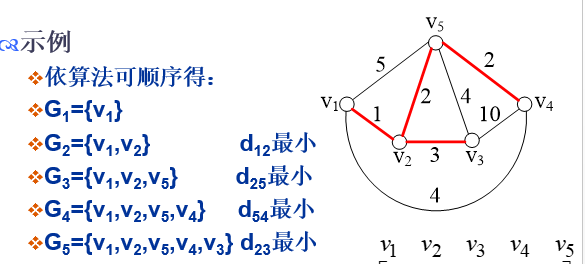
\includegraphics[width=0.7\linewidth]{figures/screenshot068}
	\caption{}
	\label{fig:screenshot068}
\end{figure}
\subsubsubsection{K算法}
\begin{figure}[H]
	\centering
	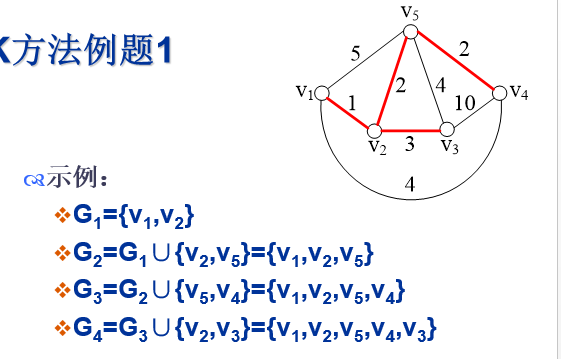
\includegraphics[width=0.7\linewidth]{figures/screenshot069}
	\caption{}
	\label{fig:screenshot069}
\end{figure}
\subsubsubsection{破圈法}
\begin{figure}[H]
	\centering
	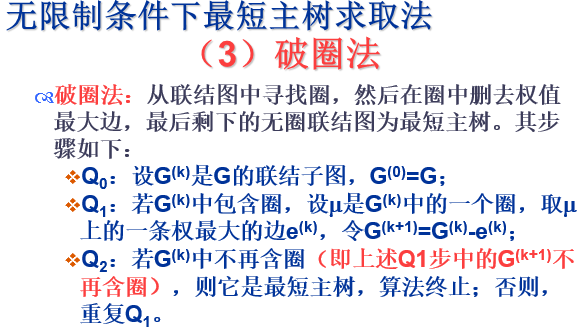
\includegraphics[width=0.7\linewidth]{figures/screenshot070}
	\caption{}
	\label{fig:screenshot070}
\end{figure}
\subsubsection{有限制条件下最短树的求取
}
\subsubsubsection{穷举法(可用置换法)
}

\subsubsubsection{E-W算法}
\subsection{端间的最短径}
\subsubsection{D算法}
\begin{figure}[H]
	\centering
	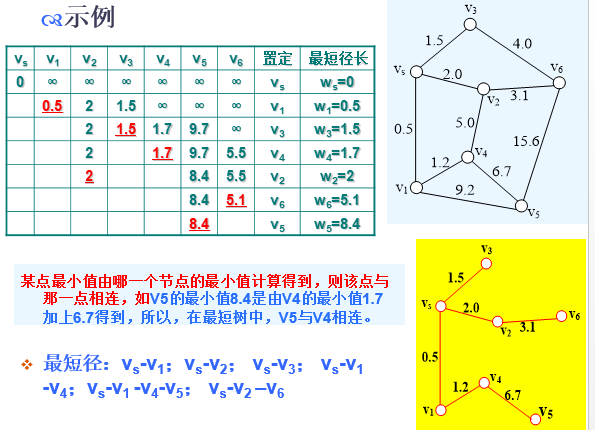
\includegraphics[width=0.7\linewidth]{figures/screenshot071}
	\caption{}
	\label{fig:screenshot071}
\end{figure}
\subsubsection{F算法}
十字交叉法,加上一个中转矩阵(每次更新时,更新中转矩阵即可)
\subsection{次短径和可用径
}
\begin{figure}[H]
	\centering
	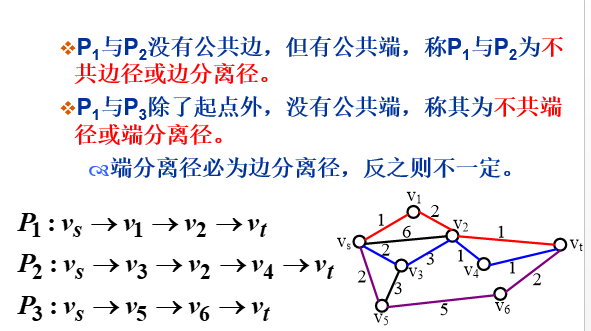
\includegraphics[width=0.7\linewidth]{figures/screenshot072}
	\caption{}
	\label{fig:screenshot072}
\end{figure}
\subsubsection{找与最短径边分离的次短径}
当用F算法或D算法得到最短径后\textbf{,从原图中去掉此径的所有边(保留这边的两个端}),然后在剩下的图中\textbf{用D算法求vs和vt间的最短径}。这就是所要求的次短径。这方法还可继续下去。
\subsubsection{找与最短径端分离的最短径。
}
在这种情况下,求得最短径后\textbf{,应把径中的所有中间端去掉(同时也去掉与之关联的边)},在余下的图中求vs和vt间最短径,就得到与最短径分离的次短径。这方法也可继续下去。
\subsection{限制条件下的可用径}
\begin{enumerate}
	\item 用F算法求得图的最短径长矩阵W和转接矩阵R
	\item DFS遍历各点,在进行判定。
\end{enumerate}
\begin{figure}[H]
	\centering
	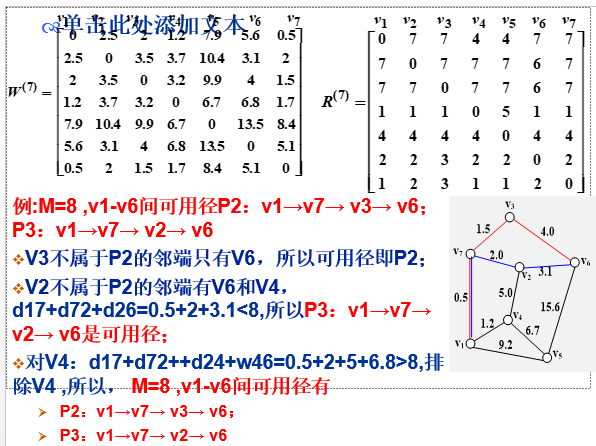
\includegraphics[width=0.7\linewidth]{figures/screenshot073}
	\caption{}
	\label{fig:screenshot073}
\end{figure}
\section{网的中心和中点}
\subsection{网中心}
Steps:
\begin{itemize}
	\item wij有一最大值;称为最长的最短径.\textbf{求每个端点到其它端点的最大长度}
	\item ti的最小值所对应的端vi*称为网的中心.求上述长度的最小值,所对应的点设置为中心。
\end{itemize}
\begin{figure}[H]
	\centering
	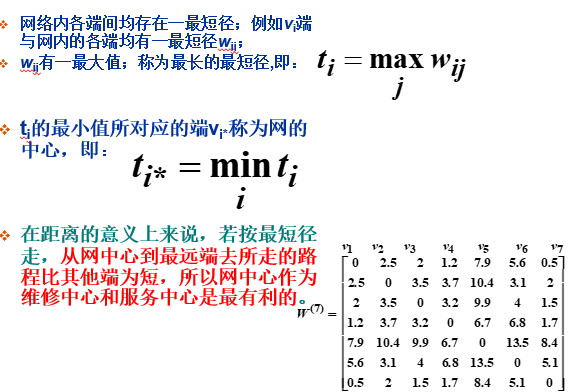
\includegraphics[width=0.7\linewidth]{figures/screenshot074}
	\caption{}
	\label{fig:screenshot074}
\end{figure}
\subsection{网中点}
Steps:
\begin{itemize}
	\item 按行求和
	\item 上述的最小值所对应的点
\end{itemize}
\textbf{网的中点可用作全网的交换或控制中心}
\begin{figure}[H]
	\centering
	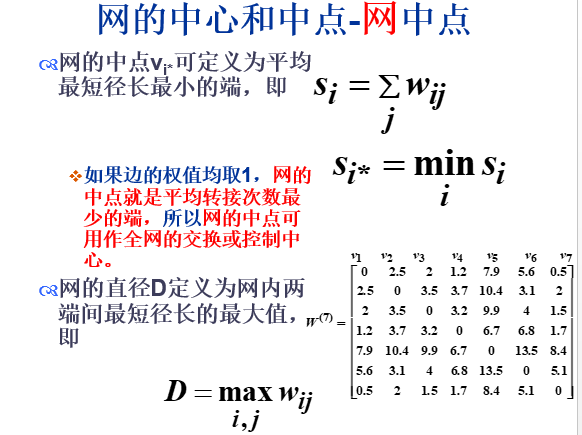
\includegraphics[width=0.7\linewidth]{figures/screenshot075}
	\caption{}
	\label{fig:screenshot075}
\end{figure}
例题:
\begin{figure}[H]
	\centering
	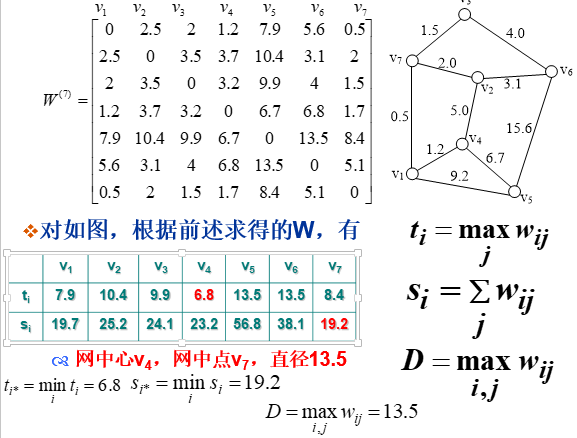
\includegraphics[width=0.7\linewidth]{figures/screenshot076}
	\caption{}
	\label{fig:screenshot076}
\end{figure}
\section{站址问题}
\subsection{单中点问题
}
设有n个用户点,它们的平面坐标分别为(xi,yi)(i=1,2,…,n)。又设各点的加权系数为wi,代表用户所需的联线数或其它需求的大小。单中点问题就是要找到一个中点的坐标(xq,yq),使代价L最小。
\begin{equation}\label{key}
L = \sum{i}{} w_id_i
\end{equation}
$ d_i $为距离的测度
\begin{enumerate}
	\item 欧式距离,平方和求根
	\item 距离平方,欧式距离的平方。适合电磁场传播
	\item 矩形距离,直角边的距离。适合城市街道铺设
\end{enumerate}
\textbf{欧式距离或者平方下},中心站点的最小距离几何确定法:\\
可以证明,中点的位置,是距离三个点位置最近的中心点,按照初等几何的原理,应该是该点与三个点的连线形成的夹角,均为120度。
\begin{figure}[H]
	\centering
	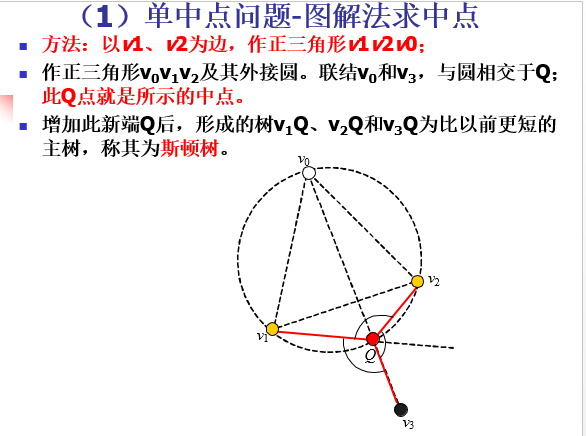
\includegraphics[width=0.7\linewidth]{figures/screenshot077}
	\caption{}
	\label{fig:screenshot077}
\end{figure}
斯顿树:如容许增加新的端点,包括中心点,存在比以前的最短主树更短的主树。这种主树称为斯顿树。\\
\vspace{1pt}
\textbf{矩形线距离的情况}
理论基础:
\begin{figure}[H]
	\centering
	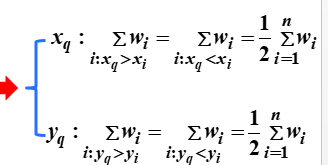
\includegraphics[width=0.7\linewidth]{figures/screenshot078}
	\caption{}
	\label{fig:screenshot078}
\end{figure}
几种情况:
\begin{figure}[H]
	\centering
	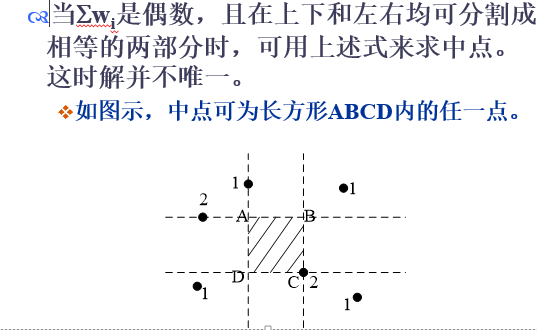
\includegraphics[width=0.7\linewidth]{figures/screenshot079}
	\caption{}
	\label{fig:screenshot079}
\end{figure}
\begin{figure}[H]
	\centering
	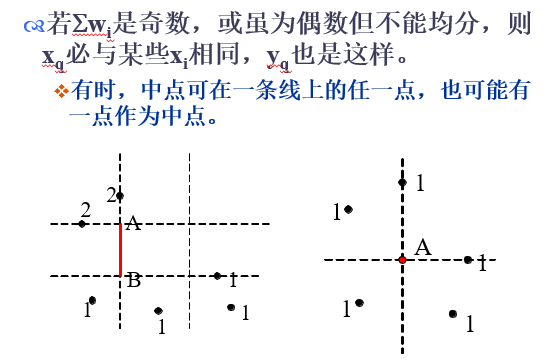
\includegraphics[width=0.7\linewidth]{figures/screenshot080}
	\caption{}
	\label{fig:screenshot080}
\end{figure}

\subsection{k中点问题}
一般所谓的k中点问题,是指k为预给值,\textbf{不计各中点的中继线代价,求这些中点的位置,以使总代价最小}。
\begin{equation}\label{key}
L = \sum_{i,j}^{} c_{ij}w_jd_j
\end{equation}
$ c_{ij} $表示i,j是否有连接。
类似\textbf{k-means}算法。先随机确定初始点,之后根据测度进行k聚类,更新中点,判定误差。
\subsection{设站问题}
\begin{figure}[H]
	\centering
	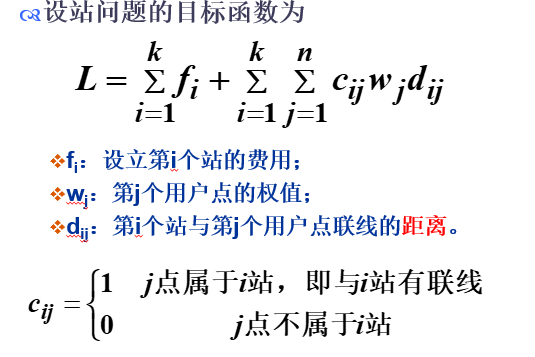
\includegraphics[width=0.7\linewidth]{figures/screenshot081}
	\caption{}
	\label{fig:screenshot081}
\end{figure}
单,双,三中点分别计算。得到一个关于设站成本f的图形。再进一步分析
\begin{figure}[H]
	\centering
	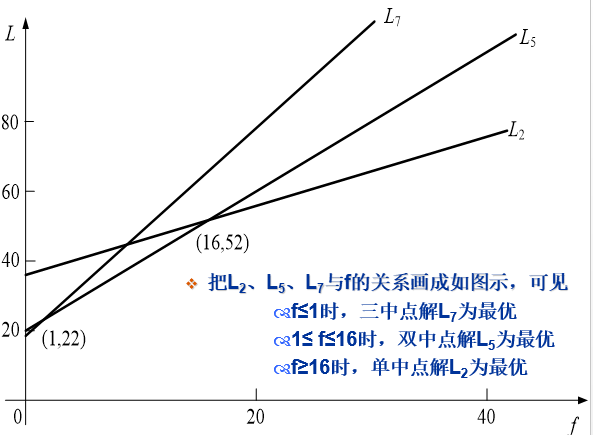
\includegraphics[width=0.7\linewidth]{figures/screenshot082}
	\caption{}
	\label{fig:screenshot082}
\end{figure}








